\documentclass[10pt]{article}
\usepackage[margin=0.9in]{geometry}
\usepackage{amsmath,amssymb,booktabs,graphicx,hyperref,xcolor,caption,subcaption}
\usepackage[numbers]{natbib}
\newcommand{\pend}[1]{\textcolor{red}{#1}}
\captionsetup{font=small}
\newcommand{\bottle}{\textsc{BoTTLE}}

\title{\bottle: Predicting the Cost per Successful Task of Robot Foundation Models\\on Hardware You Do Not Own}
\author{Prashanth Kumar Murali}
\date{}

\begin{document}
\maketitle

\begin{abstract}
Vision-language-action (VLA) models are usually compared by task success rate, and occasionally by
inference latency on one GPU. Neither answers the deployment question: \emph{what does one
successful task cost on a given device?} Answering it today requires owning every candidate
device. We present \bottle{} (\textbf{B}enchmark \textbf{o}f \textbf{T}ask-level \textbf{T}otal
\textbf{L}atency \& \textbf{E}nergy), an open-source framework and CLI that (i) predicts per-call
VLA latency and energy on unowned hardware from a per-stage roofline model, (ii) calibrates it with
a single measurement on any available device, and (iii) converts the result into time, energy and
dollars per \emph{successful} episode, accounting for action chunking, synchronous vs.\ asynchronous
execution, retries and robot-side costs. Validating against 31 published latencies of eight VLA
variants on nine devices, we find that published eager-mode latencies are dominated by time a
roofline cannot explain (geometric mean $2.4\times$ the roofline); a naive single-factor
calibration therefore \emph{worsens} transfer to Jetson devices (63\% MAPE). Overhead-aware
calibration, which transfers the unexplained time as an additive residual rather than scaling it
with accelerator throughput, reduces cross-device error to 28\% MAPE (95\% CI 19--36\%, resampling
source groups), against a measured software-stack spread of up to $1.95\times$ for the same model
and device. Applying \bottle{} to LIBERO with Monte Carlo uncertainty propagation, we show that
(a) a software-stack choice that reorders latency rankings on 6 of 9 devices leaves the cheapest
model per success unchanged, (b) counting compute only, a \$249 Jetson Orin Nano is the cheapest
device with probability $>0.99$ for every model that fits, but once robot time is billed desktop
GPUs win, and (c) the long-horizon suite costs $2.4$--$4.3\times$ more per success than the
spatial suite. A closed-loop simulation with emulated device latency shows that
E3's latency-independent success holds up to Thor's 308\,ms per chunk, but success falls by about
13 points at ${\sim}630$\,ms and to zero at 1{,}500\,ms, where stalls exhaust the episode's time
budget. \bottle{} runs on a laptop or free Colab GPU and requires no hardware purchase.
\end{abstract}

\section{Introduction}
Robot foundation models are moving from research demos to deployment on embedded computers such as
NVIDIA Jetson Thor and Orin. Practitioners must choose a \emph{(model, device, precision,
execution mode)} configuration, but the evidence available is fragmented: model papers report
success rates on simulated benchmarks such as LIBERO~\citep{liu2023libero} and a latency on one
desktop or datacenter GPU~\citep{kim2024openvla,kim2025oft,black2024pi0}; recent systems studies
measure latency breakdowns on edge hardware~\citep{xu2026hwbench,waseem2026where} but do not
predict unmeasured configurations and do not connect latency to task outcomes.

Two observations motivate this work. First, what a deployer pays for is a \emph{successful
task}: a policy that is 2$\times$ faster but fails twice as often is not cheaper, and in
synchronous control the robot idles while the policy thinks, so latency multiplies robot time.
This is the robotics analogue of cost-aware agent evaluation~\citep{kapoor2024agents}. Second,
the people making the decision frequently do not own the target device. Analytical roofline
models~\citep{williams2009roofline,yuan2024llmviewer,sun2026codesign} predict LLM inference
from datasheets, but, as we show, raw VLA deployments in eager PyTorch run far from the roofline,
so spec-only prediction is off by $>2\times$ on average.

\paragraph{Contributions.}
\begin{enumerate}
\item \bottle, an open-source framework and CLI (installable as \texttt{bottle-bench}) with
per-stage roofline models of eight VLAs (OpenVLA, OpenVLA-OFT, $\pi_0$, $\pi_{0.5}$, SmolVLA,
GR00T N1.5, N1.6 and N1.7) and 13 devices, a shape-faithful synthetic profiler for CUDA, MPS and CPU, and a
task-level cost model (\S\ref{sec:method}).
\item \emph{Overhead-aware calibration}: carrying the time a roofline cannot explain on the
reference device to the target as an additive residual (optionally scaled by a host-CPU prior)
instead of scaling it with accelerator throughput. On 32 published cross-device pairs from 8
source groups it reduces mean absolute percentage error (MAPE) from 48.8\% for single-factor
calibration to 28.1\% (\S\ref{sec:e2}).
\item A cost-per-success study of six VLAs on LIBERO across nine devices and three cost regimes,
with uncertainty propagated from the predictor's measured error, success-rate sampling, assumed
horizons and prices, reporting only rankings that survive it (\S\ref{sec:e3}).
\item A curated dataset of 31 published VLA latency measurements with sources and settings,
released with the tool.
\item A closed-loop LIBERO study that emulates target-device latency in simulation with no target
hardware: SmolVLA's success is unchanged up to Thor's 308\,ms per chunk, drops by ${\sim}13$
points at ${\sim}630$\,ms and reaches zero at 1{,}500\,ms, mainly by exhausting the task's time
budget (\S\ref{sec:e4}).
\end{enumerate}

\section{Related Work}
\paragraph{VLA models and efficiency.} OpenVLA~\citep{kim2024openvla} decodes one action token per
dimension autoregressively; OpenVLA-OFT~\citep{kim2025oft} replaces this with parallel decoding of
action chunks, reporting $26\times$ higher throughput; $\pi_0$/$\pi_{0.5}$~\citep{black2024pi0,pi2025pi05}
and GR00T~\citep{nvidia2025gr00t} use flow-matching action experts conditioned on a VLM prefix;
SmolVLA~\citep{shukor2025smolvla} targets affordable hardware.
\paragraph{VLA systems measurement.} VLA-HWBench~\citep{xu2026hwbench} profiles 18 VLAs on Jetson
Thor and attributes time to pipeline stages; \citet{waseem2026where} study bottlenecks and
optimization interactions across GPUs, including energy on Thor. Both are measurement studies;
\bottle{} is complementary, using their data for validation and predicting configurations not
measured.
\paragraph{Performance and cost modelling.} Roofline models~\citep{williams2009roofline} underlie
LLM inference analyzers~\citep{yuan2024llmviewer} and hardware co-design~\citep{sun2026codesign}.
Zeus~\citep{you2023zeus} measures and optimizes GPU energy. \citet{kapoor2024agents} argue for
cost-accuracy Pareto evaluation of AI agents. To our knowledge, no prior work combines success
rate, retries, control-loop timing, energy and dollars into a per-successful-task metric for
robot policies, or predicts it for unowned hardware.

\section{Method}\label{sec:method}
\subsection{Per-stage roofline model}
A VLA call is a sequence of stages (vision encoder(s), VLM prefill, action head), each a stack of
$L$ transformer layers of width $d$, MLP width $d_\text{ff}$ and KV width $d_\text{kv}$, processing
$T$ tokens and repeated $R$ times (e.g.\ 7 autoregressive token steps for OpenVLA, 10 denoising
steps for $\pi_0$, 4 for GR00T). Action stages attend to a cached prefix of $S$ tokens. Per layer we
count parameters $P = 2d^2 + 2dd_\text{kv} + c\,d\,d_\text{ff}$ ($c{=}3$ gated, $2$ GELU) and
\begin{align}
F &= 2PT + 4TSd, &
B &= P\,w_b + T(8d + 3d_\text{ff})\,a_b + 2Sd_\text{kv}a_b,
\end{align}
with $w_b,a_b$ the weight and activation bytes of the precision. Stage time is
\begin{equation}
t = R\left[\max\!\left(\frac{LF}{\eta_c\,\Pi_p},\ \frac{LB}{\eta_m\,\beta}\right) + 12L\,\tau_\text{launch}\right],
\end{equation}
where $\Pi_p$ is the device peak at precision $p$, $\beta$ the memory bandwidth, $\eta_c{=}0.5$,
$\eta_m{=}0.75$ default efficiencies and $\tau_\text{launch}$ the per-kernel launch overhead. Call
latency is $\ell = \sum_s t_s + h/\sigma$, a host term $h$ scaled by relative host-CPU speed
$\sigma$. Power is $P_\text{idle} + u(P_\text{TDP}-P_\text{idle})$ with utilization $u$; memory
footprint is $1.1\times$ weights $+$ KV $+$ 0.5\,GB.

\subsection{Calibration from one measurement}
Given a measured latency $m$ on a reference device $r$ and roofline predictions $\hat\ell_r$,
$\hat\ell_t$ on reference and target, \emph{global} calibration predicts
$\ell_t = \hat\ell_t\, m/\hat\ell_r$ (and \emph{stage} calibration does the same per stage when
stage times are available). This assumes the gap to the roofline is a fixed fraction of compute
time. Our measurements contradict this: eager VLA stacks spend most of their time in Python
dispatch, small-kernel launches, synchronizations and pre/post-processing, which scale with the
\emph{host CPU}, not with accelerator FLOPs or bandwidth. \emph{Overhead-aware} calibration
therefore splits the measurement into an accelerator part and an unexplained residual, which is
added to the target rather than scaled:
\begin{equation}
\ell_t = \min\!\left(\tfrac{m}{\hat\ell_r},1\right)\hat\ell_t + \max(m-\hat\ell_r,0)\,\frac{\sigma_r}{\sigma_t}.
\end{equation}
Host-speed priors $\sigma$ are set from CPU class (1.0 for modern x86 server cores, 0.75 for Thor's
Neoverse-V3AE, 0.45 for Orin's Cortex-A78AE, 0.35 for Orin Nano, 0.8 for T4 cloud hosts, 1.2
for desktop CPUs), not fitted to the validation data. With $\sigma_r{=}\sigma_t$ the method reduces
to a constant additive residual, which we report as an ablation (\S\ref{sec:e2}). We interpret the
residual as host and framework overhead, but our validation tests only that it transfers
additively, not its cause. When the residual instead reflects accelerator inefficiency on a
slow reference (e.g.\ an A10G calibrating an H100), it is carried to the target unscaled and the
method overpredicts.

\subsection{Task-level cost}
A task attempt needs $N$ control steps at rate $f$; the model emits chunks of $H_\text{chunk}$
actions of which $H \le H_\text{chunk}$ are executed per call, so there are $C=\lceil N/H\rceil$
calls. Attempt duration is
\begin{equation}
D_\text{sync} = \frac{N}{f} + C\ell, \qquad D_\text{async} = \max\!\left(\frac{N}{f},\,C\ell\right) + \ell,
\end{equation}
and asynchronous execution is real-time iff $\ell \le H/f$. Energy per attempt is
$C\ell P + (D - C\ell)P_\text{idle} + D\,P_\text{robot}$; dollars are energy $\times$ electricity price
plus $D\times$(device rate $+$ robot/operator rate), with the device rate being purchase price
amortized over lifetime $\times$ duty cycle (or a cloud hourly price). With per-attempt success
probability $p$, the expected number of attempts is $1/p$, so every per-success quantity is the
per-attempt quantity divided by $p$. \bottle{} reports these per configuration together with the
cost--success Pareto front over configurations that are real-time and fit in memory.

\subsection{Implementation}
\bottle{} is a dependency-free Python package with optional PyTorch (profiling) and NVML (energy)
extras. The CLI provides \texttt{hw}, \texttt{models}, \texttt{estimate}, \texttt{profile},
\texttt{probe} (microbenchmarks peak FLOPs, bandwidth and launch overhead of the local device),
\texttt{task}, \texttt{sweep} and \texttt{validate}. Devices and models are extensible via JSON.
The profiler builds synthetic, shape-faithful transformer blocks (GQA, SDPA, cached prefix, gated
or GELU MLP) for each stage, so a profile needs no model weights, checkpoints or licenses. A Colab
notebook profiles on a free T4 and runs a calibrated sweep.

\section{Experiments}
\subsection{E1: Local cross-device transfer}\label{sec:e1}
To test the predictor end to end with measurements we control, we use the only hardware available
to us: an Apple M5 laptop (16\,GB unified memory). \texttt{bottle probe} measures its peaks
(GPU via Metal/MPS: 12.1 fp16 / 2.9 fp32 TFLOPS, 121\,GB/s; CPU: 2.1 fp32 TFLOPS, 127\,GB/s),
which define three ``devices'': CPU fp32, GPU fp32 and GPU fp16. We profile all eight VLA presets
on each with the synthetic profiler (models above 1B parameters are profiled on 4 layers per stage
on the GPU and 2 on the CPU, then extrapolated per layer), and predict every device from every
other (48 predictions per calibrated predictor), including cross-precision transfer.

\begin{table}[h]\centering\small
\begin{tabular}{lrr}
\toprule
Predictor & MAPE & median APE \\
\midrule
Roofline, ideal efficiency & 36.6\% & 34.1\% \\
Roofline, default efficiency & 31.8\% & 31.6\% \\
Global calibration & 31.5\% & 27.2\% \\
Stage calibration & 29.5\% & 25.3\% \\
Overhead-aware calibration (\textbf{ours}) & 26.2\% & 21.1\% \\
\bottomrule
\end{tabular}

\caption{E1: latency prediction across the three local Apple M5 configurations (8 VLAs).}\label{tab:local}
\end{table}

Table~\ref{tab:local} shows that with probed specs the roofline alone is already within 32\% MAPE
(19.5\% on CPU, 29.2\% GPU fp16, 46.6\% GPU fp32), because the synthetic profiler runs pure
transformer stacks with little host overhead. Calibration helps modestly, and overhead-aware
calibration is best (26.2\%). The largest difference appears in cross-precision transfer: from
GPU fp16 to GPU fp32, global calibration errs by 57.3\% and overhead-aware by 24.8\%, because
the fp16 run's fixed overheads do not slow down with fp32 arithmetic. Two caveats bound this
experiment. First, layer extrapolation itself costs accuracy: SmolVLA on GPU fp16 extrapolated
from 2 layers is 27\% off its full-depth measurement. Second, the laptop is a shared, unmanaged
machine: the same full-depth SmolVLA fp16 configuration measured 104\,ms and 167\,ms in two runs
under different memory pressure, a run-to-run spread comparable to the prediction error.
E1 therefore shows that the pipeline works on a no-cost device and that overhead-aware
calibration is not worse than the alternatives when overhead is small; the decisive test is E2.


\subsection{E2: Validation against published measurements}\label{sec:e2}
We collected 31 published batch-1 latencies (Appendix~\ref{app:data}) for eight VLA variants on
nine devices from model papers, the Isaac-GR00T repository~\citep{isaacgr00t} and two systems
studies~\citep{waseem2026where,xu2026hwbench}. Measurements are grouped by source and setting;
calibration transfers only within a group, from a non-Jetson reference to every other device
(32 ordered pairs, 18 with Jetson targets). Pairs within a group share measurements and are not
independent, and two GR00T groups contribute 18 of the 32; we therefore report 95\% confidence
intervals from a bootstrap over the 8 groups, a group-averaged MAPE, and per-group results
(Appendix Table~\ref{tab:groups}). No parameter is fitted to these data, so there is no
train/test split to leak, but the method was designed after seeing them; the results should be
read as a retrospective validation.

\paragraph{The roofline gap.} Spec-only predictions underpredict with a geometric-mean ratio of
0.41 and are within $2\times$ for only 13 of 31 cases (42\%); the worst is $14\times$ too fast. The gap is not uniform: the JAX-compiled $\pi_0$
on an RTX~4090 is predicted within 2\% (71.8 vs.\ 73\,ms), whereas the eager GR00T~N1.6 backbone
on H100 measures 23\,ms against a 3.2\,ms roofline, and SmolVLA (0.45B) takes 208\,ms on an H100
NVL against a 15\,ms roofline. A slower Jetson Thor runs SmolVLA in only 1.5$\times$ the H100 time
despite $3.2\times$ less compute and $14\times$ less bandwidth---the signature of host-bound
execution.

\begin{table}[t]\centering\small
\begin{tabular}{lrrrrrr}
\toprule
Predictor & MAPE [95\% CI] & Group MAPE & Median & Jetson & $\le$25\% & $\le$2$\times$ \\
\midrule
Same latency as reference & 59.9 [38, 94] & 57.6 & 48.0 & 50.8 & 25\% & 59\% \\
Spec-only roofline & 51.8 [35, 68] & 55.1 & 55.7 & 54.0 & 6\% & 44\% \\
Global calibration & 48.8 [37, 73] & 60.0 & 36.3 & 63.3 & 34\% & 88\% \\
Additive residual (no host prior) & 32.8 [27, 40] & 31.0 & 31.2 & 33.4 & 41\% & 84\% \\
Overhead-aware (\textbf{ours}) & 28.1 [19, 36] & 23.5 & 22.7 & 27.7 & 56\% & 100\% \\
\bottomrule
\end{tabular}

\caption{Cross-device latency transfer on 32 published (reference$\to$target) pairs from 8 source
groups. MAPE in \%; CI: 95\% bootstrap over source groups; Group MAPE: mean of per-group MAPEs;
Jetson: MAPE on the 18 Jetson targets; $\le$25\%: share of pairs with APE $\le 25\%$;
$\le2\times$: share with $0.5 \le$ pred/meas $\le 2$. Additive residual is our method with all
host priors equal.}\label{tab:transfer}
\end{table}

\begin{figure}[t]\centering
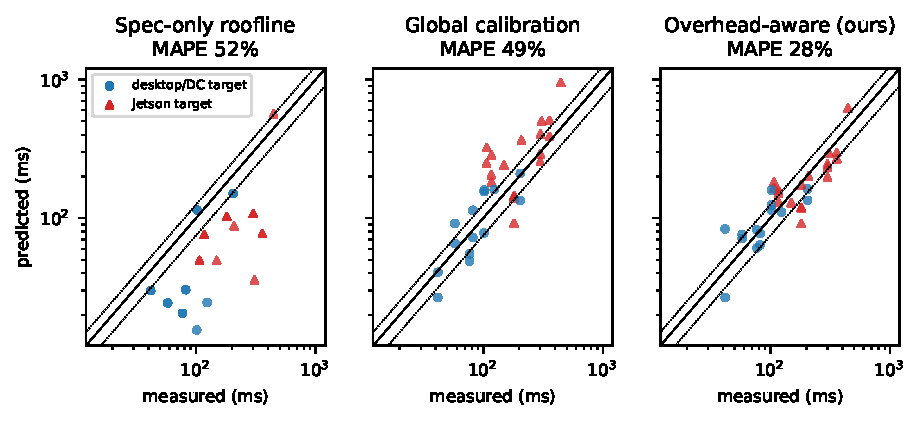
\includegraphics[width=\linewidth]{figs/transfer.pdf}
\caption{Predicted vs.\ measured latency for the 32 transfer pairs. Dotted: $\pm25\%$. Global
calibration scales host overhead by accelerator throughput and overpredicts Jetson latency;
overhead-aware calibration does not.}\label{fig:transfer}
\end{figure}

\paragraph{Transfer.} Table~\ref{tab:transfer} and Figure~\ref{fig:transfer} compare five
predictors. Single-factor calibration helps desktop-to-desktop transfer but \emph{hurts} on
Jetson targets (63.3\% vs.\ 54.0\% spec-only): it multiplies tens of milliseconds of host overhead
by the $4$--$20\times$ accelerator slowdown. Overhead-aware calibration reduces MAPE to 28.1\%
overall (95\% CI 19--36\%) and 27.7\% on Jetson, with median 22.7\% and 56\% of predictions
within 25\%. Its improvement over global calibration is $-20.7$ points (95\% CI $-48$ to $-3$),
and it beats global calibration in 6 of 8 groups. It loses in the two OpenVLA-OFT groups
(34.1\% vs.\ 19.8\% on a single pair; 39.5\% vs.\ 30.7\% with fused attention), the latter driven
by the A10G$\to$H100 pair (100\% APE), the accelerator-inefficiency failure mode described in
\S\ref{sec:method}.

\paragraph{Most of the gain is the additive form, not the host prior.} With all host priors
equal (a constant additive residual) MAPE is 32.8\% (33.4\% Jetson). The registry priors improve
this by 4.7 points (95\% CI 2.4--8.6). Perturbing the Jetson priors gives 31.4\% ($\times0.75$),
28.5\% ($\times1.25$) and 30.3\% (halfway to 1). All variants stay well below global calibration;
the host prior is a secondary refinement.

\paragraph{Noise floor.} The same model on the same device differs across sources by up to
$1.95\times$ ($\pi_{0.5}$ on Thor: 208 vs.\ 405\,ms), $1.38\times$ (OpenVLA-OFT on Thor) and
$1.40\times$ (GR00T N1.7 on Thor). Any predictor that ignores the software stack is bounded by
this spread. A 28\% transfer error is of the same order, which suggests that further gains
require calibrating on the \emph{same software stack} that will be deployed, as \bottle{}
recommends, rather than a better device model.

\paragraph{Energy.} \citet{waseem2026where} report energy per inference on Thor for five VLAs,
implying average module power of 24--79\,W. The default utilization prior ($u{=}0.6$, 86\,W)
overpredicts energy by 107\% MAPE; calibrating $u$ from the other four models (leave-one-out)
reduces this to 39\% (per model: 2\% OpenVLA, 4\% GR00T N1.7, 13\% $\pi_{0.5}$, 49\% OFT, 126\%
SmolVLA). Host-bound inference draws far below TDP, so energy, like latency, needs one calibration
point; E3 therefore samples $u\in[0.2,1]$ rather than relying on the default.

\subsection{E3: Cost per successful LIBERO task}\label{sec:e3}
\paragraph{Setup.} We combine published LIBERO success rates per suite (Appendix
Table~\ref{tab:success}; averages OpenVLA 76.5\%, OpenVLA-OFT 97.1\%, $\pi_0$ 94.2\%, $\pi_{0.5}$
96.9\%, SmolVLA 87.2\%, GR00T N1.6 97.0\%) with per-call latencies. Where the source used to anchor a
model also reports the target device, we use that measurement (9 of 54 cells, marked * in
Table~\ref{tab:latency}); otherwise we use overhead-calibrated predictions anchored on one
published \emph{eager PyTorch} measurement per model on a non-Jetson GPU. $\pi_0$ has no published
eager measurement; we anchor it on the eager $\pi_{0.5}$ H100 NVL measurement scaled by the
roofline ratio of the two models, which share backbone and action expert. LIBERO runs at 20\,Hz
with maximum episode lengths of 220/280/300/520 steps (spatial/object/goal/long) plus 10 settle
steps; failed attempts run to the limit. Execution horizons follow the published evaluation code
($H{=}1$ OpenVLA, 8 OFT and GR00T, 5 $\pi_0$/$\pi_{0.5}$); SmolVLA's is not documented and is
swept. Point estimates use 60\% of the step limit for successful episodes, 3-year amortization at
50\% duty, \$0.15/kWh, and three regimes: \emph{compute only}; \emph{+robot} (\$5/h amortized
robot, 150\,W); \emph{+robot+operator} (\$35/h).

\paragraph{Uncertainty.} Point estimates hide that many cost differences are smaller than the
predictor's error. We therefore run 2{,}000 Monte Carlo draws that jointly sample: latency
multipliers from the 32 empirical E2 log-residuals of overhead-aware calibration (or
$\pm15\%$ lognormal for measured cells); per-suite success rates from Beta posteriors given the
published trial counts; SmolVLA's horizon from $\{5,10,25,50\}$; the successful-episode fraction
from $[0.4,0.8]$; power utilization $u\in[0.2,1]$; electricity \$0.08--0.30/kWh; lifetime 2--5
years and duty 25--75\%; robot \$2.5--10/h and operator \$20--50/h; and a 0--30\,ms network round
trip for server-class GPUs (H100, A10G, L4, T4). We call a configuration the \emph{robust} winner
only if it is cheapest in $\ge80\%$ of draws.

\begin{table}[t]\centering\small\setlength{\tabcolsep}{3pt}
\begin{tabular}{l r rrrrrrrrr}
\toprule
Model & SR & H100 & 5090 & 4090 & A10G & L4 & T4 & Thor & AGX Orin & Orin Nano \\
\midrule
\multicolumn{11}{l}{\emph{compute only}} \\
OpenVLA & 76.5 & 37.0 & 4.17 & 4.39 & 11.4 & 12.0 & -- & 13.9 & 15.8 & -- \\
OpenVLA-OFT & 97.1 & \textbf{7.72} & 0.64 & \underline{0.54} & 1.20 & 0.85 & -- & 1.22 & 1.04 & -- \\
$\pi_0$ & 94.2 & 11.2 & 0.88 & 0.73 & 1.61 & 1.16 & 1.10 & 1.66 & 1.47 & \underline{0.31} \\
$\pi_{0.5}$ & 96.9 & 10.3 & 0.80 & 0.66 & 1.46 & 1.05 & 0.98 & 1.56 & 1.30 & \underline{0.26} \\
SmolVLA & 87.2 & 12.7 & 0.90 & 0.72 & 1.56 & 1.10 & 0.95 & 1.72 & 1.22 & \underline{0.19} \\
GR00T N1.6 & 97.0 & 8.43 & \textbf{0.57} & \textbf{0.49} & 1.05 & 0.78 & \textbf{0.64} & \textbf{1.08} & 0.84 & \underline{0.12} \\
\midrule
\multicolumn{11}{l}{\emph{+ robot (\$5/h, 150 W)}} \\
OpenVLA & 76.5 & 117 & 112 & 145 & 209 & 317 & -- & 264 & 516 & -- \\
OpenVLA-OFT & 97.1 & \textbf{24.6} & 20.0 & 20.8 & 22.9 & 22.7 & -- & 23.6 & 34.3 & -- \\
$\pi_0$ & 94.2 & 35.5 & 26.3 & 27.0 & 30.5 & 31.1 & 36.3 & 32.2 & 48.6 & 73.1 \\
$\pi_{0.5}$ & 96.9 & 32.8 & 24.0 & 24.6 & 27.6 & 28.2 & 32.4 & 30.1 & 43.0 & 63.0 \\
SmolVLA & 87.2 & 40.5 & 27.5 & 27.4 & 29.8 & 29.5 & 31.6 & 33.4 & 40.3 & 46.3 \\
GR00T N1.6 & 97.0 & 26.8 & \underline{\textbf{18.2}} & \textbf{19.1} & 20.3 & 21.0 & \textbf{21.4} & \textbf{21.0} & 27.9 & 29.5 \\
\midrule
\multicolumn{11}{l}{\emph{+ robot + operator (\$35/h)}} \\
OpenVLA & 76.5 & 592 & 757 & 986 & 1388 & 2141 & -- & 1758 & 3507 & -- \\
OpenVLA-OFT & 97.1 & \textbf{125} & 135 & 141 & 153 & 153 & -- & 157 & 233 & -- \\
$\pi_0$ & 94.2 & 181 & 178 & 184 & 203 & 210 & 246 & 214 & 330 & 508 \\
$\pi_{0.5}$ & 96.9 & 167 & 163 & 168 & 184 & 190 & 220 & 201 & 292 & 438 \\
SmolVLA & 87.2 & 206 & 186 & 187 & 198 & 199 & 214 & 223 & 273 & 322 \\
GR00T N1.6 & 97.0 & 137 & \underline{\textbf{124}} & \textbf{130} & 136 & 142 & \textbf{146} & \textbf{140} & 190 & 205 \\
\bottomrule
\end{tabular}

\caption{Dollars per 1{,}000 successful LIBERO episodes (point estimates; synchronous execution,
mean over four suites). SR: average success rate (\%). \textbf{Bold}: cheapest model on that device
in $\ge$80\% of Monte Carlo draws; \underline{underline}: cheapest device for that model in
$\ge$80\% of draws; unmarked columns/rows have no robust winner. --: does not fit in device
memory.}\label{tab:cost}
\end{table}

\begin{table}[t]\centering\small\setlength{\tabcolsep}{3.5pt}
\begin{tabular}{lrrrrrrrrr}
\toprule
Model & H100 & 5090 & 4090 & A10G & L4 & T4 & Thor & AGX Orin & Orin Nano \\
\midrule
OpenVLA & 108$^\dagger$ & 164$^\dagger$ & 229$^\dagger$ & 341$^\dagger$ & 554$^\dagger$ & -- & 445*$^\dagger$ & 941$^\dagger$ & -- \\
OpenVLA-OFT & 39 & 102 & 125 & 163 & 168 & -- & 181* & 460$^\dagger$ & -- \\
$\pi_0$ & 117 & 133 & 147 & 186 & 201 & 280$^\dagger$ & 210 & 460$^\dagger$ & 846$^\dagger$ \\
$\pi_{0.5}$ & 111 & 123 & 135 & 171 & 185 & 254$^\dagger$ & 208* & 418$^\dagger$ & 755$^\dagger$ \\
SmolVLA & 208 & 180 & 182 & 221 & 227 & 281 & 308* & 493 & 669$^\dagger$ \\
GR00T N1.6 & 77* & 58* & 82* & 100 & 123 & 138 & 117* & 300* & 358 \\
\bottomrule
\end{tabular}

\caption{Per-call latency (ms, bf16, eager PyTorch). *: published measurement; others: overhead-
calibrated prediction. $^\dagger$: not real-time in asynchronous mode at 20\,Hz ($\ell > H/f$),
so the robot stalls between chunks.}\label{tab:latency}
\end{table}

\paragraph{The software stack reorders latency, not cost per success.} With all models on eager
PyTorch, the fastest model is also the cheapest per success on every device (Kendall's $\tau$
between latency and cost 0.33--1.0). Anchoring $\pi_0$ instead on its published JAX-compiled
4090 measurement makes it the fastest model on 6 of 9 devices, yet the cheapest model per success
is unchanged on all nine: GR00T N1.6 or OpenVLA-OFT, which execute 8 actions per call (vs.\ 5)
and fail less often. The robust winners (Table~\ref{tab:cost}, bold) are OpenVLA-OFT on H100
($P{=}0.98$) and GR00T N1.6 on the RTX 5090, RTX 4090, T4 and Thor ($P{=}0.83$--$0.96$). On the
A10G, L4, AGX Orin and Orin Nano no model wins robustly; on the two Orins GR00T N1.6 and SmolVLA
are not separated ($P{=}0.57$--$0.69$ vs.\ $0.31$--$0.33$), because SmolVLA's undocumented horizon
dominates its cost.

\paragraph{The optimal device depends on who pays for what.} Counting compute only, the \$249
Orin Nano is the cheapest device for every model that fits in its 8\,GB ($P{>}0.99$), by
$2.4$--$4.1\times$ in the point estimate, despite being the slowest. Once robot time is billed,
synchronous execution makes latency expensive (Figure~\ref{fig:scen}) and a tethered desktop GPU
wins: the RTX 4090 or 5090 is cheapest in 80--99\% of draws for every model except OpenVLA, but
which of the two is only resolved for GR00T N1.6 (5090, $P{=}0.92$). With an operator in the loop
the H100 becomes the most likely winner for OpenVLA and OpenVLA-OFT ($P{=}0.64$, $0.67$), not a
robust one. These are statements about the cost model under stated price ranges; they are not
validated against a measured deployment bill.

\begin{figure}[t]\centering
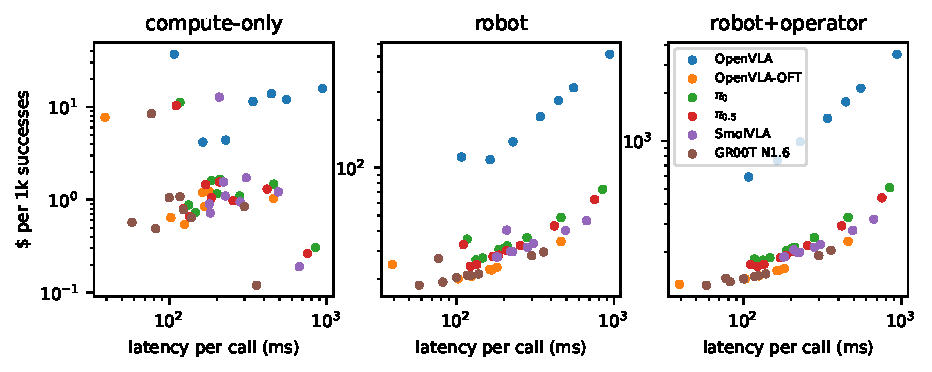
\includegraphics[width=\linewidth]{figs/scenarios.pdf}
\caption{Latency vs.\ cost per 1{,}000 successes for every (model, device) that fits in memory
(synchronous, mean over LIBERO suites, point estimates). Counting compute only, cheap slow devices
win; once robot time is billed, cost increases with latency within each model.}\label{fig:scen}
\end{figure}

\paragraph{Embedded feasibility.} OpenVLA is never real-time at 20\,Hz (single-action
decoding). On AGX Orin only SmolVLA and GR00T N1.6 are real-time; on Orin Nano only GR00T N1.6
(358\,ms predicted against a 400\,ms budget, inside the predictor's error).
Jetson Thor makes OpenVLA-OFT, $\pi_0$ and $\pi_{0.5}$ real-time.

\paragraph{Long horizons dominate.} On Thor, LIBERO-Long costs $2.4$--$4.3\times$ more per
success than LIBERO-Spatial (OpenVLA highest), from longer episodes compounded by lower success.
This ratio depends only on episode lengths and success rates, not on the latency predictor.

\subsection{E4: Does latency change success? Closed-loop simulation}\label{sec:e4}
E3, like every published LIBERO number, assumes the simulator waits for the policy. On a real
robot it does not, so we test that assumption directly, without target hardware, by emulating
each device's latency inside the simulator.

\paragraph{Setup.} We run the released \texttt{lerobot/smolvla\_libero} checkpoint (fp32, as
shipped) on all 10 LIBERO-Spatial tasks via LeRobot on a Colab T4, executing $H{=}10$ actions per
chunk at 20\,Hz (E3's synchronous setting). A thin wrapper around \texttt{lerobot-eval}
(\texttt{experiments/sim/bottle\_libero\_eval.py}) emulates a target device with latency $\ell$:
each time the policy produces a new chunk, the robot holds still (zero end-effector delta, last
gripper command) for $\lceil \ell f\rceil$ physics steps while the scene keeps evolving, and the
holds count against the episode's step budget. We compare \emph{stock} evaluation (physics paused,
$\ell{=}0$) with $\ell$ set to the T4's own per-call time measured online, to \bottle's prediction
for an RTX 4090 (182\,ms), to the published Jetson Thor measurement (308\,ms~\cite{waseem2026where}),
and to a 1{,}500\,ms stress setting. Episodes use LeRobot's seeds, identical across settings
(10 per task for the first three settings, 5 for the last two). We test per-task paired
differences against stock with a task-level bootstrap and an exact sign-flip test.

\begin{table}[t]\centering\small
\caption{Closed-loop LIBERO-Spatial success of SmolVLA ($H{=}10$, synchronous) with each chunk's
inference latency emulated as robot holds. Success CIs are Wilson intervals; $\Delta$ is the mean
per-task paired difference from stock on the same tasks (task bootstrap CI; the RTX 4090's
total is over all 10 tasks, its paired difference over the 7 with per-task logs). \emph{Max
actions} is the most policy actions that fit in LeRobot's 280-step episode budget once holds are
charged against it.}\label{tab:sim}
\resizebox{\linewidth}{!}{\begin{tabular}{lrrrrcc}
\toprule
Setting & Latency & Holds & Max actions & $n$ & Success [95\% CI] & $\Delta$ vs.\ stock, same tasks [95\% CI] \\
\midrule
Stock (physics paused) & 0\,ms & 0 & 280 & 100 & 80 [71, 87] & -- \\
RTX 4090 (predicted) & 182\,ms & 4 & 200 & 100 & 77 [68, 84] & $+0$ [$-7$, $+6$] (7 tasks) \\
Thor (published) & 308\,ms & 7 & 161 & 50 & 76 [63, 86] & $-4$ [$-15$, $+9$] \\
T4, measured per call & 632\,ms & 13 & 120 & 100 & 67 [57, 75] & $-13$ [$-28$, $+1$] \\
Stress setting & 1500\,ms & 30 & 70 & 50 & 0 [0, 7] & $-80$ [$-94$, $-60$] \\
\bottomrule
\end{tabular}
}
\end{table}

\begin{figure}[t]\centering
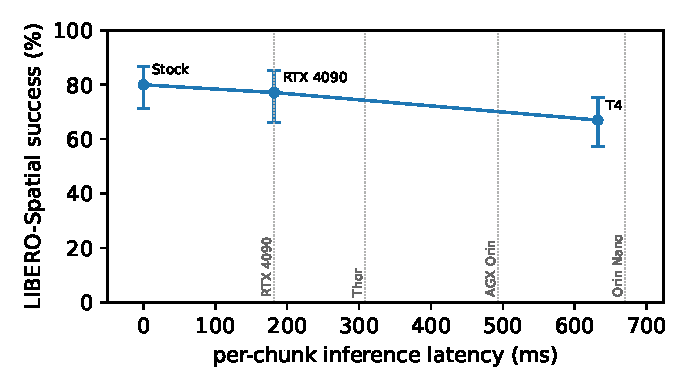
\includegraphics[width=0.75\linewidth]{figs/sim.pdf}
\caption{Closed-loop success vs.\ emulated per-chunk latency (95\% Wilson intervals). Dotted lines
mark E3's latencies for SmolVLA on edge and desktop devices.}\label{fig:sim}
\end{figure}

\paragraph{Results.} Success degrades monotonically with latency (Table~\ref{tab:sim},
Figure~\ref{fig:sim}). At the RTX 4090's predicted 182\,ms it is unchanged (77\% vs.\ 80\%;
paired $\Delta{=}0$ on the 7 tasks with per-task logs), and at Thor's published 308\,ms it is
within noise (76\%, $\Delta{=}{-}4$ points, 95\% CI $-15$ to $+9$). At the T4's measured
${\sim}630$\,ms success falls to 67\% ($\Delta{=}{-}13$, CI $-28$ to $+1$, sign-flip $p{=}0.19$),
concentrated in tasks~4 and~9, and at 1{,}500\,ms no episode succeeds (0/50, $p{=}0.004$).
The last result is mostly a \emph{time-budget} effect, not a control failure: with holds charged,
the 280-step budget leaves room for only 70 actions, fewer than a typical successful stock episode
uses. The same mechanism shrinks the budget to 130--200 actions in the other settings, so our
setup cannot yet separate ``stalls run out the clock'' from ``stalls destabilize control''; a
rerun with the budget extended by the holds would. Either way it is the deployer's question,
since real deployments also have task time limits. Combining success with time, the robot's time
per success grows from 8.8\,s (stock) to 11.4\,s (RTX 4090), 13.1\,s (Thor) and 18.4\,s (T4).
Folding the measured success loss into E3 multiplies its synchronous robot cost per success by
$s_0/s_\ell$: $1.04$ for the RTX 4090, $1.05$ for Thor, and $1.19$ at the T4's latency. This
leaves E3's desktop-GPU and Thor conclusions intact and widens the gap to devices near or beyond
${\sim}600$\,ms per chunk (Orin Nano at its predicted 669\,ms, and AGX Orin if it is
underpredicted as the T4 was).

\paragraph{A prospective latency check.} The same runs give an unplanned out-of-sample test of
the predictor. \bottle{} predicted 281\,ms for SmolVLA on a T4 in E3, which assumes half
precision; the checkpoint runs in fp32, for which it predicts 399\,ms. The measured median is
624\,ms (task medians 605--687\,ms), $1.56\times$ the fp32 prediction ($-36\%$), outside E2's
typical 28\% error but within its worst case. Part of the gap is likely Colab's two-vCPU host,
whose prior is optimistic; precision is the larger lesson: a cost prediction is only as good as
its assumption about how the model is actually deployed.

\section{Discussion and Limitations}
\textbf{Prediction is bounded by the software stack.} The dominant term in published VLA latency
is not accelerator throughput, and identical model/device pairs vary by up to $1.95\times$ across
stacks. \bottle{} therefore treats calibration on the deployed stack as first-class. Its
transfer error (median 23\%, worst case 100\%) is sufficient for ranking configurations that
differ by $2\times$ or more, but many cost comparisons in Table~\ref{tab:cost} are closer than
that, which is why we report only Monte Carlo-robust winners.
\textbf{Success is treated as independent of latency and device.} In closed-loop control, stalls
can change success; precision changes (e.g.\ INT4) can too. \bottle{} accepts per-configuration
success rates when available, but our LIBERO study uses published simulator success, in which the
environment waits for the policy, so E3 cannot capture latency-induced failures. Success rates
also come from different codebases and evaluation scripts (Table~\ref{tab:success}) and are only
approximately comparable. E4 tests the latency assumption in closed loop: it holds up to
Thor's 308\,ms, while ${\sim}630$\,ms per chunk costs about 13 points (not significant) and
1{,}500\,ms leaves too few actions in the episode budget to succeed. E4 covers one model, one suite and synchronous execution only, with 5--10
episodes per task and pure holds rather than the sensor staleness of asynchronous execution.
E3's Monte Carlo rankings do not yet include the measured $s_0/s_\ell$ correction.
\textbf{No measured bill.} Cost per success is computed, not measured end to end on a deployment.
\textbf{Approximations.} Several device peaks (A10G, Thor, Orin) and some GR00T N1.6/N1.7 and
SmolVLA dimensions are approximate; embedding tables are excluded from parameter counts; the
synthetic profiler omits tokenization and image preprocessing; host-speed priors are coarse and
the host-overhead interpretation of the residual is untested;
Apple-silicon profiles have no energy readings. Hardware prices are list prices.
\textbf{Off-board compute.} Desktop GPUs are treated as tethered; server-class GPUs receive a
0--30\,ms network round trip in the Monte Carlo only. Memory-fit predictions are not validated
against deployments.

\section{Conclusion}
Cost per successful task is the quantity robot deployers optimize, and it can be estimated without
owning the hardware---provided the estimate accounts for the host overhead that dominates today's
eager VLA stacks. \bottle{} makes this estimate one CLI command. Our study shows that the
optimal device depends on what the deployer pays for, that cost-per-success model rankings are more
stable than latency rankings across software stacks, and that many apparent differences do not
survive the uncertainty of predicting unowned hardware. Closed-loop simulation shows the
remaining assumption, that success does not depend on latency, holds at desktop-GPU and Thor speed but
fails on slow devices, which pay twice: once in stalls and again in lost successes. Code, data and
the Colab notebook are released at \url{https://github.com/PKM100/BoTTLE}.

\bibliographystyle{plainnat}
\bibliography{refs}

\appendix
\section{Published latency dataset}\label{app:data}
{\small\setlength{\tabcolsep}{4pt}\begin{tabular}{llrp{9.2cm}}
\toprule
Model & Device & ms & Source \\
\midrule
pi0 & rtx-4090 & 73 & pi0 paper arXiv 2410.24164, Table I (on-board, 3 cameras, JAX) \\
openvla & rtx-4090 & 167 & OpenVLA arXiv 2406.09246 Sec 3.5 ($\sim$6 Hz, bf16, no compile) \\
openvla & a100-40gb & 239.6 & OpenVLA-OFT arXiv 2502.19645 Table II \\
openvla-oft & a100-40gb & 112 & OpenVLA-OFT arXiv 2502.19645 Table II (wrist + proprio) \\
gr00t-n1.5 & h100-sxm & 47.88 & Isaac-GR00T n1d5 README FAQ \\
gr00t-n1.6 & rtx-5090 & 58 & Isaac-GR00T n1d6 scripts/deployment/README.md (eager) \\
gr00t-n1.6 & h100-sxm & 77 & Isaac-GR00T n1d6 scripts/deployment/README.md (eager) \\
gr00t-n1.6 & rtx-4090 & 82 & Isaac-GR00T n1d6 scripts/deployment/README.md (eager) \\
gr00t-n1.6 & jetson-agx-thor & 117 & Isaac-GR00T n1d6 scripts/deployment/README.md (eager) \\
gr00t-n1.6 & jetson-agx-orin-64gb & 300 & Isaac-GR00T n1d6 scripts/deployment/README.md (eager) \\
gr00t-n1.7 & h100-sxm & 101.5 & Isaac-GR00T main scripts/deployment/README.md (eager, incl. pre/post) \\
gr00t-n1.7 & l40 & 123.7 & Isaac-GR00T main scripts/deployment/README.md (eager, incl. pre/post) \\
gr00t-n1.7 & jetson-agx-thor & 106.8 & Isaac-GR00T main scripts/deployment/README.md (eager, incl. pre/post) \\
gr00t-n1.7 & jetson-agx-orin-64gb & 357.9 & Isaac-GR00T main scripts/deployment/README.md (eager, incl. pre/post) \\
openvla & h100-nvl & 103.8 & arXiv 2611.06710 Table 1 (eager) \\
openvla & jetson-agx-thor & 445 & arXiv 2611.06710 Table 11 (eager, MAXN) \\
openvla-oft & h100-nvl & 42.4 & arXiv 2611.06710 Table 1 (eager) \\
openvla-oft & jetson-agx-thor & 181 & arXiv 2611.06710 Table 11 (eager, MAXN) \\
pi05 & h100-nvl & 111.6 & arXiv 2611.06710 Table 1 (eager) \\
pi05 & jetson-agx-thor & 208 & arXiv 2611.06710 Table 11 (eager, MAXN) \\
gr00t-n1.7 & h100-nvl & 74.9 & arXiv 2611.06710 Table 1 (eager) \\
gr00t-n1.7 & jetson-agx-thor & 149 & arXiv 2611.06710 Table 11 (eager, MAXN) \\
smolvla & h100-nvl & 208.3 & arXiv 2611.06710 Table 1 (eager) \\
smolvla & jetson-agx-thor & 308 & arXiv 2611.06710 Table 11 (eager, MAXN) \\
openvla-oft & h100-nvl & 41.8 & arXiv 2611.06710 Table 5 (fused attention) \\
openvla-oft & a10g & 204.1 & arXiv 2611.06710 Table 5 (fused attention) \\
openvla-oft & rtx-4090 & 102.1 & arXiv 2611.06710 Table 5 (fused attention) \\
openvla-oft & jetson-agx-thor & 180.6 & arXiv 2611.06710 Table 5 (fused attention) \\
gr00t-n1.7 & jetson-agx-thor & 119 & VLA-HWBench arXiv 2610.34717 Table 7 (eager reference) \\
openvla-oft & jetson-agx-thor & 250 & VLA-HWBench arXiv 2610.34717 Table 7 (eager reference) \\
pi05 & jetson-agx-thor & 405 & VLA-HWBench arXiv 2610.34717 Table 7 (eager reference, LeRobot) \\
\bottomrule
\end{tabular}}


\section{Per-group transfer error}
\begin{table}[h]\centering\small
\begin{tabular}{lrrrrrr}
\toprule
Source group & pairs & Same & Spec & Global & Additive & Ours \\
\midrule
\texttt{gr00t-n1.6-repo} & 12 & 40 & 57 & 43 & 27 & 22 \\
\texttt{gr00t-n1.7-repo} & 6 & 33 & 71 & 73 & 33 & 32 \\
\texttt{where-openvla} & 1 & 77 & 27 & 114 & 36 & 40 \\
\texttt{where-oft} & 1 & 77 & 43 & 20 & 37 & 34 \\
\texttt{where-pi05} & 1 & 46 & 58 & 75 & 18 & 4 \\
\texttt{where-n17} & 1 & 50 & 67 & 62 & 29 & 13 \\
\texttt{where-smolvla} & 1 & 32 & 88 & 63 & 26 & 5 \\
\texttt{where-oft-fused} & 9 & 106 & 29 & 31 & 43 & 39 \\
\midrule
Group mean & & 58 & 55 & 60 & 31 & 24 \\
\bottomrule
\end{tabular}

\caption{E2 MAPE (\%) per source group. Same: reference latency reused; Spec: spec-only roofline;
Global: single-factor calibration; Additive: constant residual; Ours: overhead-aware.}\label{tab:groups}
\end{table}

\section{LIBERO success rates and execution horizons}
\begin{table}[h]\centering
{\small\setlength{\tabcolsep}{4pt}\begin{tabular}{lrrrrrrp{5.6cm}}
\toprule
Model & Spatial & Object & Goal & Long & Trials & $H$ & Source \\
\midrule
OpenVLA & 84.7 & 88.4 & 79.2 & 53.7 & 500 & 1 & OpenVLA-OFT arXiv 2502.19645 Table I (fine-tuned OpenVLA) \\
OpenVLA-OFT & 97.6 & 98.4 & 97.9 & 94.5 & 500 & 8 & OpenVLA-OFT arXiv 2502.19645 Table I \\
$\pi_0$ & 96.8 & 98.8 & 95.8 & 85.2 & 500 & 5 & OpenVLA-OFT arXiv 2502.19645 Table I (pi0 fine-tuned) \\
$\pi_{0.5}$ & 98.8 & 98.2 & 98.0 & 92.4 & 500 & 5 & openpi examples/libero/README.md (replan\_steps=5) \\
SmolVLA & 90.0 & 96.0 & 92.0 & 71.0 & 500 & 10$^\ddagger$ & SmolVLA arXiv 2506.01844 LIBERO table (0.45B) \\
GR00T N1.6 & 97.7 & 98.5 & 97.5 & 94.3 & 200 & 8 & Isaac-GR00T n1d6 examples/LIBERO/README.md \\
\bottomrule
\end{tabular}}

\caption{Per-suite LIBERO success rates (\%) and execution horizon $H$ used in E3. Trials: episodes per
suite in the source evaluation. $^\ddagger$: not documented; swept over $\{5,10,25,50\}$ in the Monte
Carlo.}\label{tab:success}
\end{table}

\end{document}
